การออกแบบ labeling tool นั้น ผู้วิจัยได้เลือกใช้แพลตฟอร์ม PyQt และภาษา Python ในการพัฒนา
เนื่องจากแพลติฟอร์ม PyQt นั้นเป็นแพลตฟอร์มที่มีผู้พัฒนาใช้กันอย่างแพร่หลาย จึงทำให้สะดวกในการศึกษาและหาข้อมูลผ่านอินเตอร์เน็ต
อีกทั้งยังเป็นแพลตฟอร์มที่สามารถพัฒนาด้วยภาษา Python ได้ และเป็นแพลตฟอร์มที่ใช้งานง่าย สามารถปรับปรุงแก้ไขได้ง่าย
เนื่องจากการสร้างแอพพลิเคชั่นนั้นจำเป็นต้องมีการปรับแก้หน้าต่างอยู่เสมอ

\subsection{แอพพลิเคชั่น labeling tool}
ภาพรวมของแอพพลิเคชั่นที่สร้างขึ้นประกอบด้วยส่วน Select, Detect, Track และ Action label
เพื่อช่วยแบ่งเบาภาระของผู้พัฒนาในการสร้าง label สำหรับสร้างโมเดลจากข้อมูลประเภทวิดีโอ โดยส่วน Select
จะต้องสามารถตัดวิดีโอส่วนที่ไม่มีมนุษย์อยู่ออกจากวิดีโอได้ Detect ต้องสามารถหาตำแหน่งของมนุษย์ภายในวิดีโอได้
Track ต้องสามารถทำนายตำแหน่งต่อไปของมนุษย์ข้อมูลตำแหน่งของมนุษย์จาก Detect ได้
Action label ต้องสามารถทำนายการกระทำของมนุษย์ได้ในระดับหนึ่ง โดยทุกส่วนการทำงานมนุษย์ต้องสามารถทำงานร่วมกับระบบได้
ดังรูปที่ \ref{fig:labeling_overview}

\begin{figure}[!ht]
    \centering
    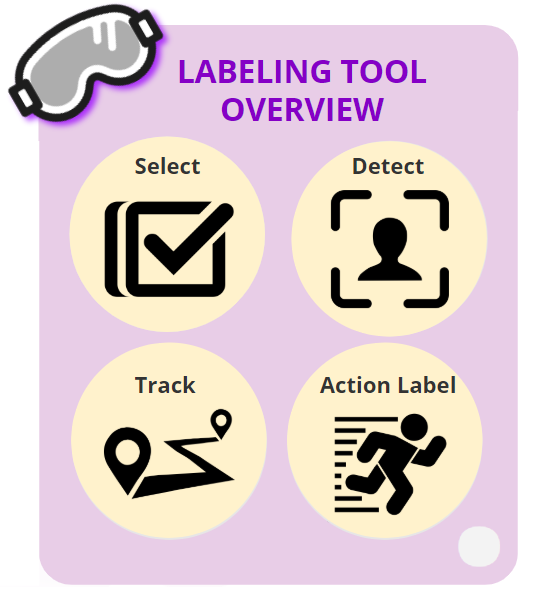
\includegraphics[width=0.7\textwidth]{chapter3/images/3_6/labelingToolOverview.png}
    \caption{ภาพรวมระบบของแอพพลิเคชั่น labeling tool}
    \label{fig:labeling_overview}
\end{figure}

\clearpage
\subsection*{โดยแต่ละส่วนจะมีรายละเอียดดังนี้}
\subsubsection{Select}
ในส่วนของแถบ Select จะมีหน้าต่างเป็นดังรูปที่ \ref{fig:selectTab} โดยในส่วนนี้จะมีหน้าที่ในการโหลดวิดีโอที่ต้องการ
กำหนดอัตราการหยิบตัวอย่างเฟรมของวิดีโอแล้วเก็บเฟรมเหล่านั้นเป็นคีย์เฟรม(Keyframe) และตัดวิดีโอส่วนที่ไม่มีมนุษย์อยู่ออกไป
\begin{figure}[!ht]
    \centering
    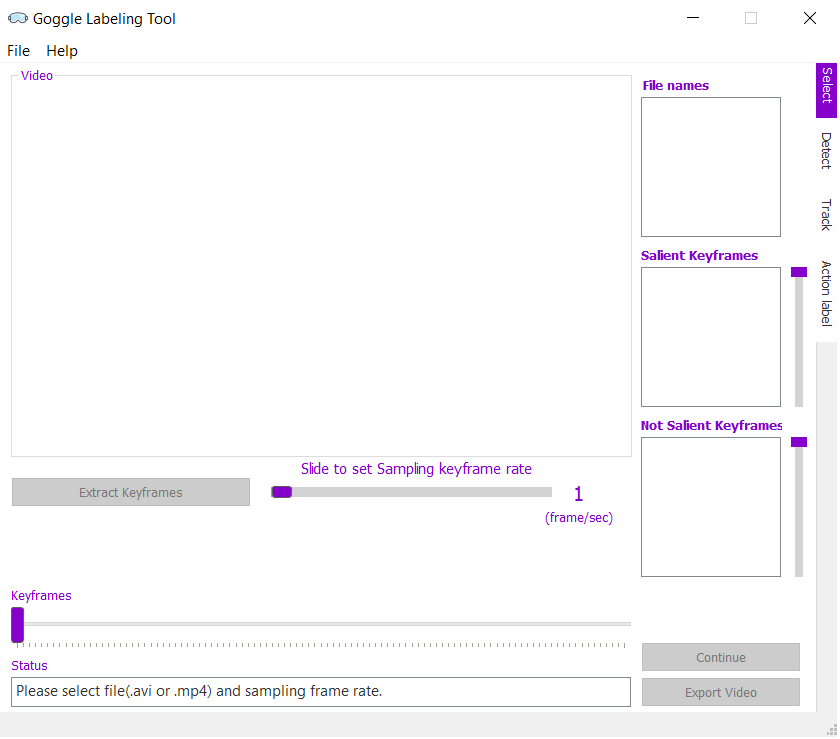
\includegraphics[width=1\textwidth]{chapter3/images/3_6/SelectTab.png}
    \caption{หน้าต่างแถบ Select ของแอพพลิเคชั่น labeling tool}
    \label{fig:selectTab}
\end{figure}
\clearpage
ซึ่งในขั้นตอนการตัดส่วนวิดีโอที่ไม่มีมนุษย์อยู่นั้น ได้ใช้โมเดล YoLo-v3 สำหรับตรวจหามนุษย์ในแต่ละคีย์เฟรม
จากนั้นจะแยกคีย์เฟรมที่มีมนุษย์อยู่ และที่ไม่มีมนุษย์อยู่ออกมา แล้วเก็บไว้ในช่องรายการหมายเลข 1 และ 2 ตามลำดับ
ดังรูปที่ \ref{fig:SelectTab_sampled}

\begin{figure}[!ht]
    \centering
    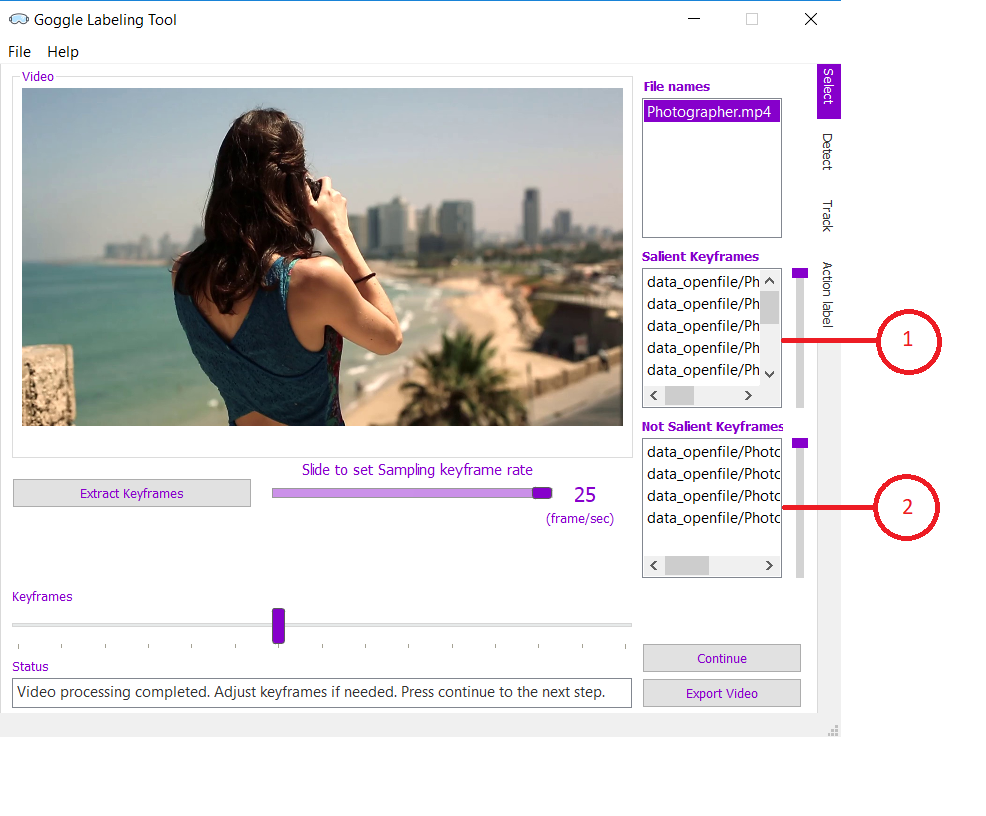
\includegraphics[width=1\textwidth]{chapter3/images/3_6/SelectTab_sampled.png}
    \caption{หลังจากตัดส่วนวิดีโอแล้ว คีย์เฟรมจะถูกเก็บไว้ในช่องรายการตามประเภท}
    \label{fig:SelectTab_sampled}
\end{figure}
\clearpage
\subsubsection{Detect}
ในส่วนของแถบ Delect จะมีหน้าต่างเป็นดังรูปที่ \ref{fig:detectTab} โดยในส่วนนี้มีหน้าที่ในการตรวจหาตำแหน่งของมนุษย์ภายในคีย์เฟรม
และสร้างกรอบสี่เหลี่ยมเพื่อแสดงถึงบริเวณที่มีมนุษย์อยู่ สามารถทำได้สองแบบ 
คือแบบอัตโนมัติ(Auto mode) และแบบทำด้วยมือ(Manual mode) 
ซึ่งในแบบอัตโนมัตินั้นจะใช้โมเดล YoLo-v3 ในการตรวจหาตำแหน่งของมนุษย์ในทุกคีย์เฟรม
และแบบทำด้วยมือ จะสามารถเพิ่ม หรือลบกรอบสี่เหลี่ยมในคีย์เฟรมได้ สามารถใช้ในการแก้ไขความผิดพลาดของแบบอัตโนมัติได้

\begin{figure}[!ht]
    \centering
    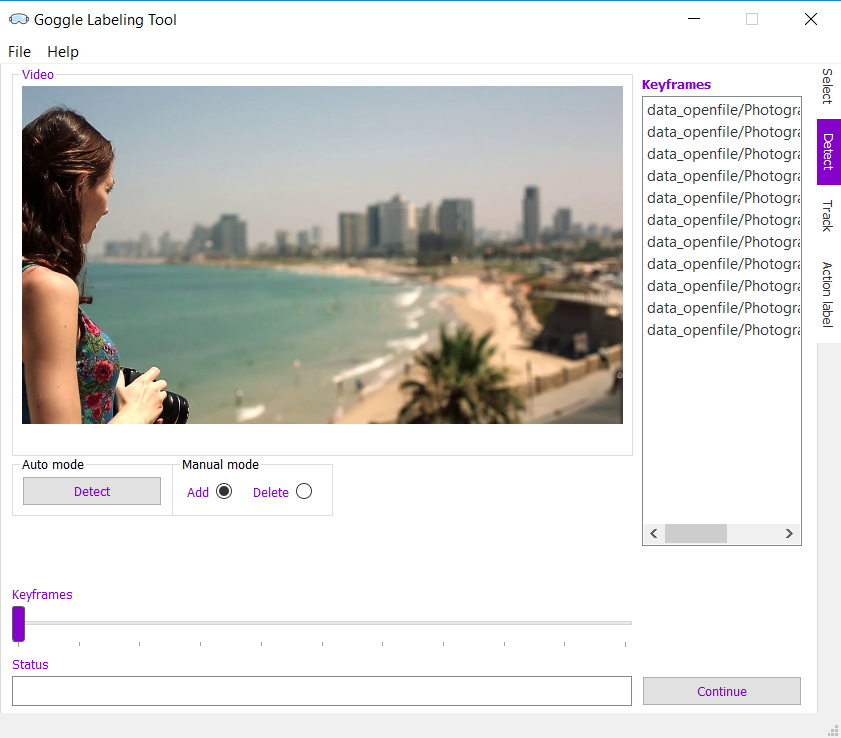
\includegraphics[width=1\textwidth]{chapter3/images/3_6/detect.png}
    \caption{หน้าต่างแถบ Detect ของแอพพลิเคชั่น labeling tool}
    \label{fig:detectTab}
\end{figure}
\clearpage
ซึ่งหลังจากที่กดปุ่ม Detect แล้วนั้นปัญญาประดิษฐ์ของ labeling tool จะทำการตรวจหาตำแหน่งของมนุษย์อัตโนมัติ
และสร้างกรอบสี่เหลี่ยมขึ้นมาครอบตำแหน่งเหล่านั้นในทุกคีย์เฟรม ดังรูปที่ \ref{fig:detectTab_detected}
\begin{figure}[!ht]
    \centering
    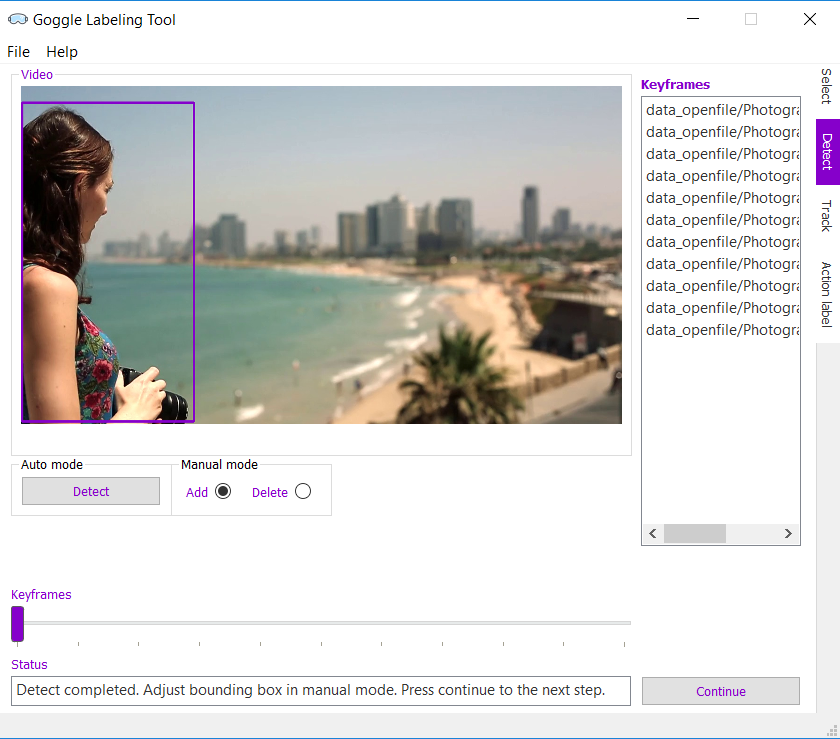
\includegraphics[width=1\textwidth]{chapter3/images/3_6/detect_complete.png}
    \caption{หลังจากกดปุ่ม Detect ระบบจะสร้างกรอบสี่เหลี่ยมขึ้นมาครอบตำแหน่งมนุษย์}
    \label{fig:detectTab_detected}
\end{figure}

ผู้ใช้สามารถตรวจสอบความถูกต้องของปัญญาประดิษฐ์ และแก้ไข(เพิ่มหรือลบ)ด้วยตัวเองได้
เพื่อเพิ่มประสิทธิภาพของชุดข้อมูลให้มากขึ้นได้ และถ้าหากพอใจกับผลลัพธ์ที่ได้แล้วก็สามารถปุ่ม
Continue เพื่อไปสู่ขั้นตอนต่อไป
\clearpage
\subsubsection{Track}
ในส่วนของแถบ Track จะมีหน้าต่างเป็นดังรูปที่ \ref{fig:trackTab} 
โดยในส่วนนี้มีหน้าที่ในการทำนายตำแหน่งต่อไปของกรอบสี่เหลี่ยมที่ได้จากคีย์เฟรมก่อนหน้าจนถึงคีย์เฟรมถัดไป
และสร้างกรอบสี่เหลี่ยมเพื่อแสดงถึงบริเวณที่มีคาดว่าจะมีมนุษย์อยู่ 
สามารถทำได้สองแบบ คือแบบอัตโนมัติ(Auto mode) และแบบทำด้วยมือ(Manual mode) 
ซึ่งในแบบอัตโนมัตินั้นจะใช้อัลกอริทึมของ dlib ในการทำนายตำแหน่งของมนุษย์ในเฟรมถัดไป 
และแบบทำด้วยมือจะสามารถเพิ่ม หรือลบกรอบสี่เหลี่ยมในเฟรมได้ 
สามารถใช้ในการแก้ไขความผิดพลาดของแบบอัตโนมัติได้
\begin{figure}[!ht]
    \centering
    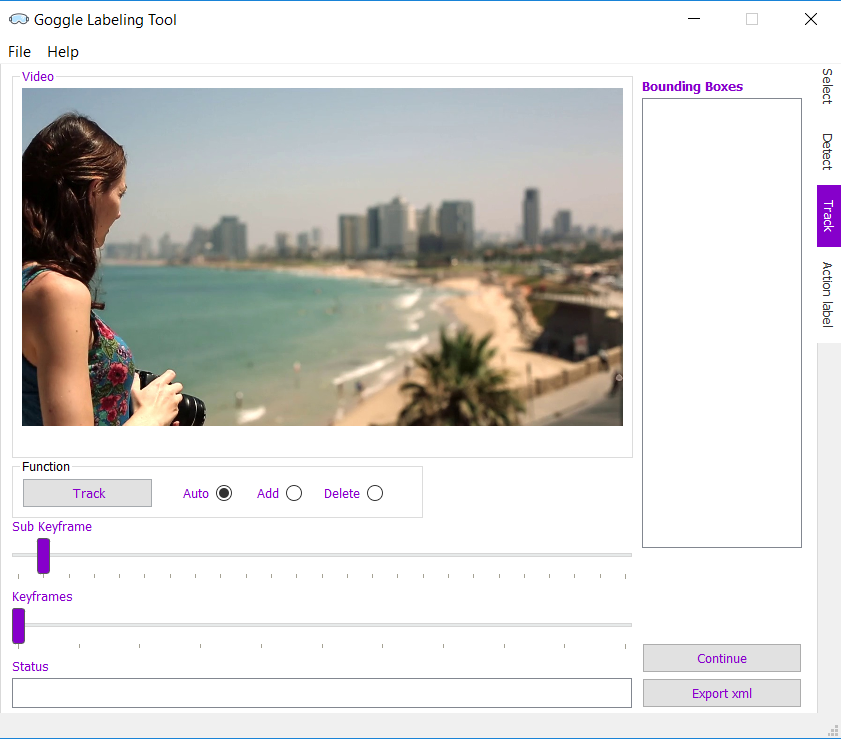
\includegraphics[width=1\textwidth]{chapter3/images/3_6/track.png}
    \caption{หน้าต่างแถบ Track ของแอพพลิเคชั่น labeling tool}
    \label{fig:trackTab}
\end{figure}
